\documentclass[twoside]{book}

% Packages required by doxygen
\usepackage{fixltx2e}
\usepackage{calc}
\usepackage{doxygen}
\usepackage{graphicx}
\usepackage[utf8]{inputenc}
\usepackage{makeidx}
\usepackage{multicol}
\usepackage{multirow}
\PassOptionsToPackage{warn}{textcomp}
\usepackage{textcomp}
\usepackage[nointegrals]{wasysym}
\usepackage[table]{xcolor}

% NLS support packages
\usepackage[french]{babel}

% Font selection
\usepackage[T1]{fontenc}
\usepackage{mathptmx}
\usepackage[scaled=.90]{helvet}
\usepackage{courier}
\usepackage{amssymb}
\usepackage{sectsty}
\renewcommand{\familydefault}{\sfdefault}
\allsectionsfont{%
  \fontseries{bc}\selectfont%
  \color{darkgray}%
}
\renewcommand{\DoxyLabelFont}{%
  \fontseries{bc}\selectfont%
  \color{darkgray}%
}
\newcommand{\+}{\discretionary{\mbox{\scriptsize$\hookleftarrow$}}{}{}}

% Page & text layout
\usepackage{geometry}
\geometry{%
  a4paper,%
  top=2.5cm,%
  bottom=2.5cm,%
  left=2.5cm,%
  right=2.5cm%
}
\tolerance=750
\hfuzz=15pt
\hbadness=750
\setlength{\emergencystretch}{15pt}
\setlength{\parindent}{0cm}
\setlength{\parskip}{0.2cm}
\makeatletter
\renewcommand{\paragraph}{%
  \@startsection{paragraph}{4}{0ex}{-1.0ex}{1.0ex}{%
    \normalfont\normalsize\bfseries\SS@parafont%
  }%
}
\renewcommand{\subparagraph}{%
  \@startsection{subparagraph}{5}{0ex}{-1.0ex}{1.0ex}{%
    \normalfont\normalsize\bfseries\SS@subparafont%
  }%
}
\makeatother

% Headers & footers
\usepackage{fancyhdr}
\pagestyle{fancyplain}
\fancyhead[LE]{\fancyplain{}{\bfseries\thepage}}
\fancyhead[CE]{\fancyplain{}{}}
\fancyhead[RE]{\fancyplain{}{\bfseries\leftmark}}
\fancyhead[LO]{\fancyplain{}{\bfseries\rightmark}}
\fancyhead[CO]{\fancyplain{}{}}
\fancyhead[RO]{\fancyplain{}{\bfseries\thepage}}
\fancyfoot[LE]{\fancyplain{}{}}
\fancyfoot[CE]{\fancyplain{}{}}
\fancyfoot[RE]{\fancyplain{}{\bfseries\scriptsize Généré le Dimanche 22 Novembre 2015 17\+:07\+:06 pour Solver de Ruzzle par Cousin Brandon/ Ngatchou Junior par Doxygen }}
\fancyfoot[LO]{\fancyplain{}{\bfseries\scriptsize Généré le Dimanche 22 Novembre 2015 17\+:07\+:06 pour Solver de Ruzzle par Cousin Brandon/ Ngatchou Junior par Doxygen }}
\fancyfoot[CO]{\fancyplain{}{}}
\fancyfoot[RO]{\fancyplain{}{}}
\renewcommand{\footrulewidth}{0.4pt}
\renewcommand{\chaptermark}[1]{%
  \markboth{#1}{}%
}
\renewcommand{\sectionmark}[1]{%
  \markright{\thesection\ #1}%
}

% Indices & bibliography
\usepackage{natbib}
\usepackage[titles]{tocloft}
\setcounter{tocdepth}{3}
\setcounter{secnumdepth}{5}
\makeindex

% Hyperlinks (required, but should be loaded last)
\usepackage{ifpdf}
\ifpdf
  \usepackage[pdftex,pagebackref=true]{hyperref}
\else
  \usepackage[ps2pdf,pagebackref=true]{hyperref}
\fi
\hypersetup{%
  colorlinks=true,%
  linkcolor=blue,%
  citecolor=blue,%
  unicode%
}

% Custom commands
\newcommand{\clearemptydoublepage}{%
  \newpage{\pagestyle{empty}\cleardoublepage}%
}


%===== C O N T E N T S =====

\begin{document}

% Titlepage & ToC
\hypersetup{pageanchor=false,
             bookmarks=true,
             bookmarksnumbered=true,
             pdfencoding=unicode
            }
\pagenumbering{roman}
\begin{titlepage}
\vspace*{7cm}
\begin{center}%
{\Large Solver de Ruzzle par Cousin Brandon/ Ngatchou Junior }\\
\vspace*{1cm}
{\large Généré par Doxygen 1.8.8}\\
\vspace*{0.5cm}
{\small Dimanche 22 Novembre 2015 17:07:06}\\
\end{center}
\end{titlepage}
\clearemptydoublepage
\tableofcontents
\clearemptydoublepage
\pagenumbering{arabic}
\hypersetup{pageanchor=true}

%--- Begin generated contents ---
\chapter{Page principale}
\label{index}\hypertarget{index}{}Le Ruzzle est un jeu originaire du monde mobile, ce jeu consiste à former le plus de mots en un temps imparti à partir d'une grille de lettres générée aléatoirement. Le but étant de marquer le plus de points possible pour celà des bonus lettre et mot double/triple sont répartis sur la grille mais il n'est pas permis de réutiliser deux fois la même case.

\section*{Instructions de compilation}

\begin{quote}
\$ make \end{quote}


Permet de compiler l'ensemble des sources, l'exécutable généré peut être retrouvé dans $\ast$$\ast$./bin$\ast$$\ast$ .

\begin{quote}
\$ make mrproper \end{quote}


Permet de nettoyer le dossier.

\section*{Utilisation}

\begin{quote}
\$ ./bin/ruzzle\+Solver \end{quote}


Permet d'exécuter le programme en générant une grille aléatoire, les lettres sont tirées au hasard en prenant compte de leurs fréquences d'apparition dans la langue française.

On peut prédéfinir une grille à l'aide d'une chaine de 16 caractères.

Par exemple\+:

\begin{quote}
\$ ./bin/ruzzle\+Solver adcksxirmdesuckh \end{quote}


Génèrera la grille \+:

\begin{quote}
A~~~~D~~~~C~~~~K

S~~~~X~~~~I~~~~R

M~~~~D~~~~E~~~~S

U~~~~C~~~~K~~~~H

\end{quote}


Dans le cas d'une chaîne trop petite un message d'erreur apparaîtra, si la chaîne est trop grande, la grille sera composée des 16 premiers caractères.

Les bonus lettres et mots sont tirés aléatoirement de manière à ce qu'il n'y ait pas trop de bonus. 
\chapter{Index des classes}
\section{Liste des classes}
Liste des classes, structures, unions et interfaces avec une brève description \-:\begin{DoxyCompactList}
\item\contentsline{section}{\hyperlink{structelement}{element} \\*Définis un élément de la liste }{\pageref{structelement}}{}
\item\contentsline{section}{\hyperlink{structt__Case}{t\-\_\-\-Case} \\*Définis une case par 4 caractéristiques }{\pageref{structt__Case}}{}
\end{DoxyCompactList}

\chapter{Index des fichiers}
\section{Liste des fichiers}
Liste de tous les fichiers documentés avec une brève description \-:\begin{DoxyCompactList}
\item\contentsline{section}{include/\hyperlink{display_8h}{display.\-h} \\*Prototype de la grille }{\pageref{display_8h}}{}
\item\contentsline{section}{include/\hyperlink{random_8h}{random.\-h} \\*Prototype de la partie aléatoire du solver }{\pageref{random_8h}}{}
\item\contentsline{section}{include/\hyperlink{solver_8h}{solver.\-h} \\*Prototype du solver }{\pageref{solver_8h}}{}
\item\contentsline{section}{include/\hyperlink{trie_8h}{trie.\-h} \\*Prototype de la liste chaînée }{\pageref{trie_8h}}{}
\item\contentsline{section}{src/\hyperlink{display_8c}{display.\-c} \\*Affiche la grille }{\pageref{display_8c}}{}
\item\contentsline{section}{src/\hyperlink{random_8c}{random.\-c} \\*Fonctions aléatoires }{\pageref{random_8c}}{}
\item\contentsline{section}{src/\hyperlink{ruzzle_8c}{ruzzle.\-c} \\*Solver de Ruzzle }{\pageref{ruzzle_8c}}{}
\item\contentsline{section}{src/\hyperlink{solver_8c}{solver.\-c} \\*Résoud la grille }{\pageref{solver_8c}}{}
\item\contentsline{section}{src/\hyperlink{trie_8c}{trie.\-c} \\*Met au point une liste chaînée d'ordre décroissant }{\pageref{trie_8c}}{}
\end{DoxyCompactList}

\chapter{Documentation des classes}
\hypertarget{structelement}{\section{Référence de la structure element}
\label{structelement}\index{element@{element}}
}


Définis un élément de la liste.  




{\ttfamily \#include $<$trie.\+h$>$}



Graphe de collaboration de element\+:\nopagebreak
\begin{figure}[H]
\begin{center}
\leavevmode
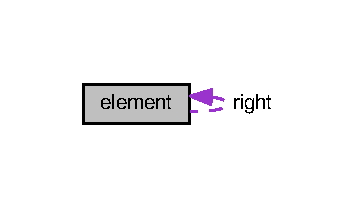
\includegraphics[width=171pt]{structelement__coll__graph}
\end{center}
\end{figure}
\subsection*{Attributs publics}
\begin{DoxyCompactItemize}
\item 
\hypertarget{structelement_af607a92824fa5d32abd559d6fefda79a}{char \hyperlink{structelement_af607a92824fa5d32abd559d6fefda79a}{word} \mbox{[}17\mbox{]}}\label{structelement_af607a92824fa5d32abd559d6fefda79a}

\begin{DoxyCompactList}\small\item\em Mot à stocker. \end{DoxyCompactList}\item 
\hypertarget{structelement_afa46df5a6444396565aa685782411b44}{int \hyperlink{structelement_afa46df5a6444396565aa685782411b44}{pts}}\label{structelement_afa46df5a6444396565aa685782411b44}

\begin{DoxyCompactList}\small\item\em Nombre de points associé \end{DoxyCompactList}\item 
\hypertarget{structelement_a37542facf22f1fffc9843c9f00be9216}{struct \hyperlink{structelement}{element} $\ast$ \hyperlink{structelement_a37542facf22f1fffc9843c9f00be9216}{right}}\label{structelement_a37542facf22f1fffc9843c9f00be9216}

\begin{DoxyCompactList}\small\item\em $\ast$right Pointeur sur l'élément suivant \end{DoxyCompactList}\end{DoxyCompactItemize}


\subsection{Description détaillée}
Définis un élément de la liste. 

Définition à la ligne 10 du fichier trie.\+h.



La documentation de cette structure a été générée à partir du fichier suivant \+:\begin{DoxyCompactItemize}
\item 
include/\hyperlink{trie_8h}{trie.\+h}\end{DoxyCompactItemize}

\hypertarget{structt__Case}{\section{Référence de la structure t\+\_\+\+Case}
\label{structt__Case}\index{t\+\_\+\+Case@{t\+\_\+\+Case}}
}


Définis une case par 4 caractéristiques.  




{\ttfamily \#include $<$display.\+h$>$}

\subsection*{Attributs publics}
\begin{DoxyCompactItemize}
\item 
\hypertarget{structt__Case_ab8d4688c0772235234ba57f91302d301}{char \hyperlink{structt__Case_ab8d4688c0772235234ba57f91302d301}{let}}\label{structt__Case_ab8d4688c0772235234ba57f91302d301}

\begin{DoxyCompactList}\small\item\em Lettre à afficher. \end{DoxyCompactList}\item 
\hypertarget{structt__Case_a0ca7fb3ede63f530b081a9ba25dd0c42}{int \hyperlink{structt__Case_a0ca7fb3ede63f530b081a9ba25dd0c42}{pts}}\label{structt__Case_a0ca7fb3ede63f530b081a9ba25dd0c42}

\begin{DoxyCompactList}\small\item\em Nombre de points associé \end{DoxyCompactList}\item 
\hypertarget{structt__Case_ac6a23400b09f5d278e5fa52bca741391}{char \hyperlink{structt__Case_ac6a23400b09f5d278e5fa52bca741391}{bo\+L} \mbox{[}3\mbox{]}}\label{structt__Case_ac6a23400b09f5d278e5fa52bca741391}

\begin{DoxyCompactList}\small\item\em Bonus sur la lettre. \end{DoxyCompactList}\item 
\hypertarget{structt__Case_a5eede5d51107927662912a5b307fe6ee}{char \hyperlink{structt__Case_a5eede5d51107927662912a5b307fe6ee}{bo\+M} \mbox{[}3\mbox{]}}\label{structt__Case_a5eede5d51107927662912a5b307fe6ee}

\begin{DoxyCompactList}\small\item\em Bonus sur le mot. \end{DoxyCompactList}\item 
\hypertarget{structt__Case_a36f323f054e3e6e6a95654b63bd90652}{int \hyperlink{structt__Case_a36f323f054e3e6e6a95654b63bd90652}{visited}}\label{structt__Case_a36f323f054e3e6e6a95654b63bd90652}

\begin{DoxyCompactList}\small\item\em Définis si une case a déjà été visitée. \end{DoxyCompactList}\end{DoxyCompactItemize}


\subsection{Description détaillée}
Définis une case par 4 caractéristiques. 

Définition à la ligne 12 du fichier display.\+h.



La documentation de cette structure a été générée à partir du fichier suivant \+:\begin{DoxyCompactItemize}
\item 
include/\hyperlink{display_8h}{display.\+h}\end{DoxyCompactItemize}

\chapter{Documentation des fichiers}
\hypertarget{display_8h}{\section{Référence du fichier include/display.h}
\label{display_8h}\index{include/display.\+h@{include/display.\+h}}
}


Prototype de la grille.  


Ce graphe montre quels fichiers incluent directement ou indirectement ce fichier \+:\nopagebreak
\begin{figure}[H]
\begin{center}
\leavevmode
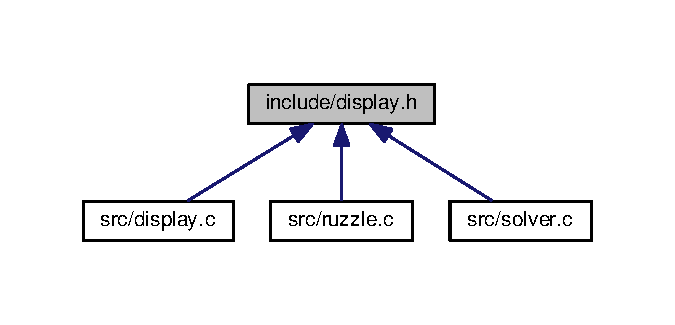
\includegraphics[width=324pt]{display_8h__dep__incl}
\end{center}
\end{figure}
\subsection*{Classes}
\begin{DoxyCompactItemize}
\item 
struct \hyperlink{structt__Case}{t\+\_\+\+Case}
\begin{DoxyCompactList}\small\item\em Définis une case par 4 caractéristiques. \end{DoxyCompactList}\end{DoxyCompactItemize}
\subsection*{Macros}
\begin{DoxyCompactItemize}
\item 
\hypertarget{display_8h_a0240ac851181b84ac374872dc5434ee4}{\#define \hyperlink{display_8h_a0240ac851181b84ac374872dc5434ee4}{N}~4}\label{display_8h_a0240ac851181b84ac374872dc5434ee4}

\begin{DoxyCompactList}\small\item\em Constante du nombre de lignes / colonnes. \end{DoxyCompactList}\end{DoxyCompactItemize}
\subsection*{Fonctions}
\begin{DoxyCompactItemize}
\item 
void \hyperlink{display_8h_a8b5a31f5bfcefe241188eca44c65834a}{Grille} (\hyperlink{structt__Case}{t\+\_\+\+Case} grid\mbox{[}\hyperlink{display_8h_a0240ac851181b84ac374872dc5434ee4}{N}\mbox{]}\mbox{[}\hyperlink{display_8h_a0240ac851181b84ac374872dc5434ee4}{N}\mbox{]}, int argc, char $\ast$grid\+Str\mbox{[}$\,$\mbox{]})
\begin{DoxyCompactList}\small\item\em Représente une grille. \end{DoxyCompactList}\end{DoxyCompactItemize}


\subsection{Description détaillée}
Prototype de la grille. 



Définition dans le fichier \hyperlink{display_8h_source}{display.\+h}.



\subsection{Documentation des fonctions}
\hypertarget{display_8h_a8b5a31f5bfcefe241188eca44c65834a}{\index{display.\+h@{display.\+h}!Grille@{Grille}}
\index{Grille@{Grille}!display.\+h@{display.\+h}}
\subsubsection[{Grille}]{\setlength{\rightskip}{0pt plus 5cm}void Grille (
\begin{DoxyParamCaption}
\item[{{\bf t\+\_\+\+Case}}]{grid\mbox{[}\+N\mbox{]}\mbox{[}\+N\mbox{]}, }
\item[{int}]{argc, }
\item[{char $\ast$}]{grid\+Str\mbox{[}$\,$\mbox{]}}
\end{DoxyParamCaption}
)}}\label{display_8h_a8b5a31f5bfcefe241188eca44c65834a}


Représente une grille. 


\begin{DoxyParams}{Paramètres}
{\em grid} & Grille à remplir \\
\hline
{\em argc} & Nombres d'arguments du main \\
\hline
{\em grid\+Str} & Grille sous forme de chaîne \\
\hline
\end{DoxyParams}


Définition à la ligne 123 du fichier display.\+c.


\hypertarget{random_8h}{\section{Référence du fichier include/random.h}
\label{random_8h}\index{include/random.\-h@{include/random.\-h}}
}


Prototype de la partie aléatoire du solver.  


Ce graphe montre quels fichiers incluent directement ou indirectement ce fichier \-:
\nopagebreak
\begin{figure}[H]
\begin{center}
\leavevmode
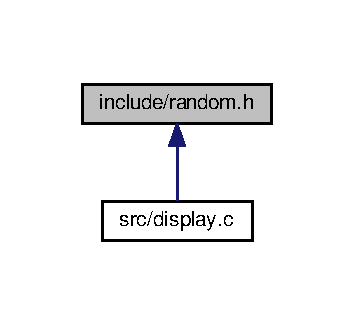
\includegraphics[width=170pt]{random_8h__dep__incl}
\end{center}
\end{figure}
\subsection*{Fonctions}
\begin{DoxyCompactItemize}
\item 
int \hyperlink{random_8h_a92316f4f4339b1dd0436637ce9552bb6}{rand\-Case} ()
\begin{DoxyCompactList}\small\item\em Permet de tirer une lettre aléatoirement. \end{DoxyCompactList}\item 
\hypertarget{random_8h_affc667f54d3aad05a212a708a1967851}{void \hyperlink{random_8h_affc667f54d3aad05a212a708a1967851}{init\-Rand} ()}\label{random_8h_affc667f54d3aad05a212a708a1967851}

\begin{DoxyCompactList}\small\item\em Initialise le tirage aléatoire. \end{DoxyCompactList}\item 
void \hyperlink{random_8h_a9b2c6b2bb8b813fc92d7f8be99e5d47d}{get\-Bonus} (char bo\-Char\-L\mbox{[}$\,$\mbox{]}, char bo\-Char\-M\mbox{[}$\,$\mbox{]}, int $\ast$nb\-\_\-bo\-L, int $\ast$nb\-\_\-bo\-M)
\begin{DoxyCompactList}\small\item\em Attribue un bonus. \end{DoxyCompactList}\item 
int \hyperlink{random_8h_a8de3f80b9cac15b21aee0c7d56ae0f5a}{get\-I\-Char} (char c)
\begin{DoxyCompactList}\small\item\em Permet de récupérer l'indice dans la matrice de la lettre tirée au hasard. \end{DoxyCompactList}\end{DoxyCompactItemize}


\subsection{Description détaillée}
Prototype de la partie aléatoire du solver. 

Définition dans le fichier \hyperlink{random_8h_source}{random.\-h}.



\subsection{Documentation des fonctions}
\hypertarget{random_8h_a9b2c6b2bb8b813fc92d7f8be99e5d47d}{\index{random.\-h@{random.\-h}!get\-Bonus@{get\-Bonus}}
\index{get\-Bonus@{get\-Bonus}!random.h@{random.\-h}}
\subsubsection[{get\-Bonus}]{\setlength{\rightskip}{0pt plus 5cm}void get\-Bonus (
\begin{DoxyParamCaption}
\item[{char}]{bo\-Char\-L\mbox{[}$\,$\mbox{]}, }
\item[{char}]{bo\-Char\-M\mbox{[}$\,$\mbox{]}, }
\item[{int $\ast$}]{nb\-\_\-bo\-L, }
\item[{int $\ast$}]{nb\-\_\-bo\-M}
\end{DoxyParamCaption}
)}}\label{random_8h_a9b2c6b2bb8b813fc92d7f8be99e5d47d}


Attribue un bonus. 


\begin{DoxyParams}{Paramètres}
{\em bo\-Char\-L\mbox{[}$\,$\mbox{]}} & Bonus lettre de la case courante \\
\hline
{\em bo\-Char\-M\mbox{[}$\,$\mbox{]}} & Bonus mot de la case courante \\
\hline
{\em nb\-\_\-bo\-L} & Nombre de bonus lettre dans la grille \\
\hline
{\em nb\-\_\-bo\-M} & Nombre de bonus mot dans la grille \\
\hline
\end{DoxyParams}


Définition à la ligne 82 du fichier random.\-c.

\hypertarget{random_8h_a8de3f80b9cac15b21aee0c7d56ae0f5a}{\index{random.\-h@{random.\-h}!get\-I\-Char@{get\-I\-Char}}
\index{get\-I\-Char@{get\-I\-Char}!random.h@{random.\-h}}
\subsubsection[{get\-I\-Char}]{\setlength{\rightskip}{0pt plus 5cm}int get\-I\-Char (
\begin{DoxyParamCaption}
\item[{char}]{c}
\end{DoxyParamCaption}
)}}\label{random_8h_a8de3f80b9cac15b21aee0c7d56ae0f5a}


Permet de récupérer l'indice dans la matrice de la lettre tirée au hasard. 


\begin{DoxyParams}{Paramètres}
{\em c} & Caractère à convertir en indice \\
\hline
\end{DoxyParams}


Définition à la ligne 63 du fichier random.\-c.

\hypertarget{random_8h_a92316f4f4339b1dd0436637ce9552bb6}{\index{random.\-h@{random.\-h}!rand\-Case@{rand\-Case}}
\index{rand\-Case@{rand\-Case}!random.h@{random.\-h}}
\subsubsection[{rand\-Case}]{\setlength{\rightskip}{0pt plus 5cm}int rand\-Case (
\begin{DoxyParamCaption}
{}
\end{DoxyParamCaption}
)}}\label{random_8h_a92316f4f4339b1dd0436637ce9552bb6}


Permet de tirer une lettre aléatoirement. 

\begin{DoxyReturn}{Renvoie}
Renvoie l'indice de la lettre tirée 
\end{DoxyReturn}


Définition à la ligne 71 du fichier random.\-c.


\hypertarget{solver_8h}{\section{Référence du fichier include/solver.h}
\label{solver_8h}\index{include/solver.\+h@{include/solver.\+h}}
}


Prototype du solver.  


Ce graphe montre quels fichiers incluent directement ou indirectement ce fichier \+:\nopagebreak
\begin{figure}[H]
\begin{center}
\leavevmode
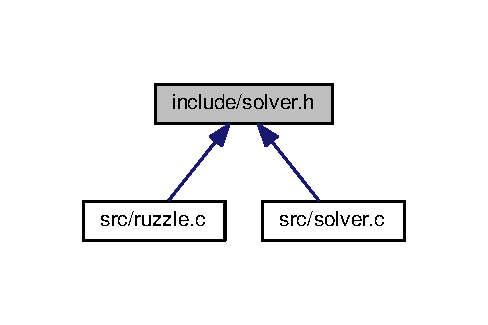
\includegraphics[width=234pt]{solver_8h__dep__incl}
\end{center}
\end{figure}
\subsection*{Fonctions}
\begin{DoxyCompactItemize}
\item 
void \hyperlink{solver_8h_acb26ab357db8918adfe55385af56ba11}{Solver} (\hyperlink{structt__Case}{t\+\_\+\+Case} grid\mbox{[}\hyperlink{display_8h_a0240ac851181b84ac374872dc5434ee4}{N}\mbox{]}\mbox{[}\hyperlink{display_8h_a0240ac851181b84ac374872dc5434ee4}{N}\mbox{]})
\begin{DoxyCompactList}\small\item\em Résoud la grille. \end{DoxyCompactList}\end{DoxyCompactItemize}


\subsection{Description détaillée}
Prototype du solver. 



Définition dans le fichier \hyperlink{solver_8h_source}{solver.\+h}.



\subsection{Documentation des fonctions}
\hypertarget{solver_8h_acb26ab357db8918adfe55385af56ba11}{\index{solver.\+h@{solver.\+h}!Solver@{Solver}}
\index{Solver@{Solver}!solver.\+h@{solver.\+h}}
\subsubsection[{Solver}]{\setlength{\rightskip}{0pt plus 5cm}void Solver (
\begin{DoxyParamCaption}
\item[{{\bf t\+\_\+\+Case}}]{grid\mbox{[}\+N\mbox{]}\mbox{[}\+N\mbox{]}}
\end{DoxyParamCaption}
)}}\label{solver_8h_acb26ab357db8918adfe55385af56ba11}


Résoud la grille. 


\begin{DoxyParams}{Paramètres}
{\em grid} & Grille à résoudre \\
\hline
\end{DoxyParams}


Définition à la ligne 148 du fichier solver.\+c.


\hypertarget{trie_8h}{\section{Référence du fichier include/trie.h}
\label{trie_8h}\index{include/trie.\+h@{include/trie.\+h}}
}


Prototype de la liste chaînée.  


Ce graphe montre quels fichiers incluent directement ou indirectement ce fichier \+:\nopagebreak
\begin{figure}[H]
\begin{center}
\leavevmode
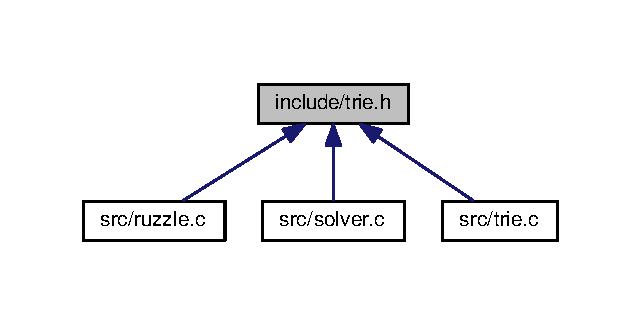
\includegraphics[width=308pt]{trie_8h__dep__incl}
\end{center}
\end{figure}
\subsection*{Classes}
\begin{DoxyCompactItemize}
\item 
struct \hyperlink{structelement}{element}
\begin{DoxyCompactList}\small\item\em Définis un élément de la liste. \end{DoxyCompactList}\end{DoxyCompactItemize}
\subsection*{Définitions de type}
\begin{DoxyCompactItemize}
\item 
typedef struct \hyperlink{structelement}{element} \hyperlink{trie_8h_aac687df386c3a390580b9fbc6fec9133}{element}
\begin{DoxyCompactList}\small\item\em Définis un élément de la liste. \end{DoxyCompactList}\end{DoxyCompactItemize}
\subsection*{Fonctions}
\begin{DoxyCompactItemize}
\item 
void \hyperlink{trie_8h_adac30872b2982daea2a38df6f042065d}{add\+Element} (\hyperlink{structelement}{element} $\ast$elem)
\begin{DoxyCompactList}\small\item\em Ajoute un élément dans la liste chaînée. \end{DoxyCompactList}\item 
\hypertarget{trie_8h_a2f736094bbaa598f70c3e241bad4a1cc}{void \hyperlink{trie_8h_a2f736094bbaa598f70c3e241bad4a1cc}{print\+List} ()}\label{trie_8h_a2f736094bbaa598f70c3e241bad4a1cc}

\begin{DoxyCompactList}\small\item\em Affiche la liste entière de la racine jusqu'à la fin. \end{DoxyCompactList}\item 
\hypertarget{trie_8h_a612285c5b9d603a0abb0feab44b8412f}{void \hyperlink{trie_8h_a612285c5b9d603a0abb0feab44b8412f}{clear\+List} ()}\label{trie_8h_a612285c5b9d603a0abb0feab44b8412f}

\begin{DoxyCompactList}\small\item\em Supprime la liste. \end{DoxyCompactList}\end{DoxyCompactItemize}


\subsection{Description détaillée}
Prototype de la liste chaînée. 



Définition dans le fichier \hyperlink{trie_8h_source}{trie.\+h}.



\subsection{Documentation des définitions de type}
\hypertarget{trie_8h_aac687df386c3a390580b9fbc6fec9133}{\index{trie.\+h@{trie.\+h}!element@{element}}
\index{element@{element}!trie.\+h@{trie.\+h}}
\subsubsection[{element}]{\setlength{\rightskip}{0pt plus 5cm}typedef struct {\bf element}  {\bf element}}}\label{trie_8h_aac687df386c3a390580b9fbc6fec9133}


Définis un élément de la liste. 



\subsection{Documentation des fonctions}
\hypertarget{trie_8h_adac30872b2982daea2a38df6f042065d}{\index{trie.\+h@{trie.\+h}!add\+Element@{add\+Element}}
\index{add\+Element@{add\+Element}!trie.\+h@{trie.\+h}}
\subsubsection[{add\+Element}]{\setlength{\rightskip}{0pt plus 5cm}void add\+Element (
\begin{DoxyParamCaption}
\item[{{\bf element} $\ast$}]{elem}
\end{DoxyParamCaption}
)}}\label{trie_8h_adac30872b2982daea2a38df6f042065d}


Ajoute un élément dans la liste chaînée. 


\begin{DoxyParams}{Paramètres}
{\em elem} & Elément à ajouter \\
\hline
\end{DoxyParams}


Définition à la ligne 20 du fichier trie.\+c.


\hypertarget{display_8c}{\section{Référence du fichier src/display.c}
\label{display_8c}\index{src/display.\+c@{src/display.\+c}}
}


Affiche la grille.  


{\ttfamily \#include $<$stdio.\+h$>$}\\*
{\ttfamily \#include $<$stdlib.\+h$>$}\\*
{\ttfamily \#include $<$string.\+h$>$}\\*
{\ttfamily \#include \char`\"{}../include/random.\+h\char`\"{}}\\*
{\ttfamily \#include \char`\"{}../include/display.\+h\char`\"{}}\\*
Graphe des dépendances par inclusion de display.\+c\+:\nopagebreak
\begin{figure}[H]
\begin{center}
\leavevmode
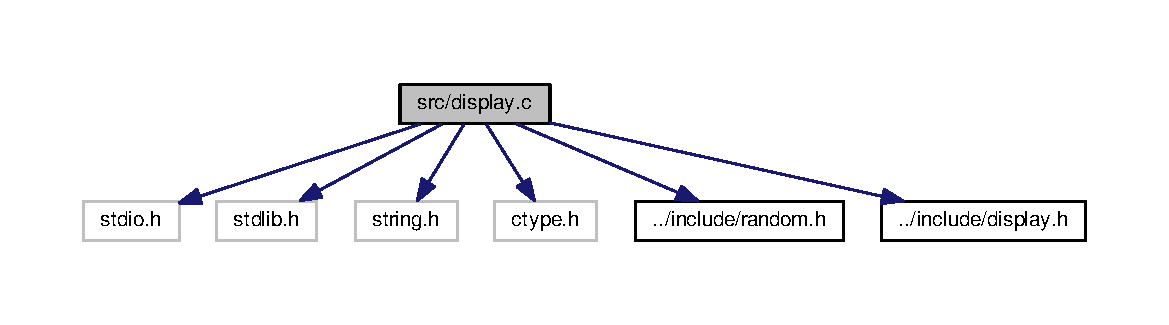
\includegraphics[width=350pt]{display_8c__incl}
\end{center}
\end{figure}
\subsection*{Fonctions}
\begin{DoxyCompactItemize}
\item 
void \hyperlink{display_8c_aa10159fb9d4c4dd0d90f094038cb8f16}{init\+Grid} (\hyperlink{structt__Case}{t\+\_\+\+Case} grid\mbox{[}\hyperlink{display_8h_a0240ac851181b84ac374872dc5434ee4}{N}\mbox{]}\mbox{[}\hyperlink{display_8h_a0240ac851181b84ac374872dc5434ee4}{N}\mbox{]})
\begin{DoxyCompactList}\small\item\em Initialise les bonus à zéros. \end{DoxyCompactList}\item 
void \hyperlink{display_8c_a996285d53053a7448de2cd3e89cc66f7}{get\+Case} (\hyperlink{structt__Case}{t\+\_\+\+Case} grid\mbox{[}\hyperlink{display_8h_a0240ac851181b84ac374872dc5434ee4}{N}\mbox{]}\mbox{[}\hyperlink{display_8h_a0240ac851181b84ac374872dc5434ee4}{N}\mbox{]}, int line, int col, int nb\+\_\+bonus\mbox{[}$\,$\mbox{]})
\begin{DoxyCompactList}\small\item\em Représente une case aléatoirement. \end{DoxyCompactList}\item 
void \hyperlink{display_8c_a369551137b4051ed8b2fd56838e8c30a}{get\+Case\+From\+Str} (\hyperlink{structt__Case}{t\+\_\+\+Case} grid\mbox{[}\hyperlink{display_8h_a0240ac851181b84ac374872dc5434ee4}{N}\mbox{]}\mbox{[}\hyperlink{display_8h_a0240ac851181b84ac374872dc5434ee4}{N}\mbox{]}, int nb\+\_\+bonus\mbox{[}$\,$\mbox{]}, char grid\+Str\mbox{[}$\,$\mbox{]}, int str\+Index)
\begin{DoxyCompactList}\small\item\em Représente une case en fonction de la chaîne tapée en paramètre de main. \end{DoxyCompactList}\item 
void \hyperlink{display_8c_a8b5a31f5bfcefe241188eca44c65834a}{Grille} (\hyperlink{structt__Case}{t\+\_\+\+Case} grid\mbox{[}\hyperlink{display_8h_a0240ac851181b84ac374872dc5434ee4}{N}\mbox{]}\mbox{[}\hyperlink{display_8h_a0240ac851181b84ac374872dc5434ee4}{N}\mbox{]}, int argc, char $\ast$grid\+Str\mbox{[}$\,$\mbox{]})
\begin{DoxyCompactList}\small\item\em Représente une grille. \end{DoxyCompactList}\end{DoxyCompactItemize}
\subsection*{Variables}
\begin{DoxyCompactItemize}
\item 
\hyperlink{structt__Case}{t\+\_\+\+Case} \hyperlink{display_8c_adc2d3888a0c89764f0fb62c303df9f6b}{alpha} \mbox{[}26\mbox{]}
\begin{DoxyCompactList}\small\item\em Définis l'alphabet et le poids de chaque lettre. \end{DoxyCompactList}\end{DoxyCompactItemize}


\subsection{Description détaillée}
Affiche la grille. 

\begin{DoxyAuthor}{Auteur}
Cousin Brandon Ngatchou Junior 
\end{DoxyAuthor}
\begin{DoxyVersion}{Version}
v1.\+00 
\end{DoxyVersion}
\begin{DoxyDate}{Date}
05/11/2015 
\end{DoxyDate}


Définition dans le fichier \hyperlink{display_8c_source}{display.\+c}.



\subsection{Documentation des fonctions}
\hypertarget{display_8c_a996285d53053a7448de2cd3e89cc66f7}{\index{display.\+c@{display.\+c}!get\+Case@{get\+Case}}
\index{get\+Case@{get\+Case}!display.\+c@{display.\+c}}
\subsubsection[{get\+Case}]{\setlength{\rightskip}{0pt plus 5cm}void get\+Case (
\begin{DoxyParamCaption}
\item[{{\bf t\+\_\+\+Case}}]{grid\mbox{[}\+N\mbox{]}\mbox{[}\+N\mbox{]}, }
\item[{int}]{line, }
\item[{int}]{col, }
\item[{int}]{nb\+\_\+bonus\mbox{[}$\,$\mbox{]}}
\end{DoxyParamCaption}
)}}\label{display_8c_a996285d53053a7448de2cd3e89cc66f7}


Représente une case aléatoirement. 


\begin{DoxyParams}{Paramètres}
{\em grid} & Grille à remplir \\
\hline
{\em line} & Ligne de la case à remplir \\
\hline
{\em col} & Colonne de la case à remplir \\
\hline
{\em nb\+\_\+bonus} & Nombre de bonus lettre et mot dans la grille \\
\hline
\end{DoxyParams}


Définition à la ligne 54 du fichier display.\+c.

\hypertarget{display_8c_a369551137b4051ed8b2fd56838e8c30a}{\index{display.\+c@{display.\+c}!get\+Case\+From\+Str@{get\+Case\+From\+Str}}
\index{get\+Case\+From\+Str@{get\+Case\+From\+Str}!display.\+c@{display.\+c}}
\subsubsection[{get\+Case\+From\+Str}]{\setlength{\rightskip}{0pt plus 5cm}void get\+Case\+From\+Str (
\begin{DoxyParamCaption}
\item[{{\bf t\+\_\+\+Case}}]{grid\mbox{[}\+N\mbox{]}\mbox{[}\+N\mbox{]}, }
\item[{int}]{nb\+\_\+bonus\mbox{[}$\,$\mbox{]}, }
\item[{char}]{grid\+Str\mbox{[}$\,$\mbox{]}, }
\item[{int}]{str\+Index}
\end{DoxyParamCaption}
)}}\label{display_8c_a369551137b4051ed8b2fd56838e8c30a}


Représente une case en fonction de la chaîne tapée en paramètre de main. 


\begin{DoxyParams}{Paramètres}
{\em grid} & Grille à remplir \\
\hline
{\em nb\+\_\+bonus} & Nombre de bonus lettre et mot dans la grille \\
\hline
{\em grid\+Str} & Chaîne de caractère passé en paramètre \\
\hline
{\em str\+Index} & Indice courant de la chaîne passée en paramètre \\
\hline
\end{DoxyParams}


Définition à la ligne 83 du fichier display.\+c.

\hypertarget{display_8c_a8b5a31f5bfcefe241188eca44c65834a}{\index{display.\+c@{display.\+c}!Grille@{Grille}}
\index{Grille@{Grille}!display.\+c@{display.\+c}}
\subsubsection[{Grille}]{\setlength{\rightskip}{0pt plus 5cm}void Grille (
\begin{DoxyParamCaption}
\item[{{\bf t\+\_\+\+Case}}]{grid\mbox{[}\+N\mbox{]}\mbox{[}\+N\mbox{]}, }
\item[{int}]{argc, }
\item[{char $\ast$}]{grid\+Str\mbox{[}$\,$\mbox{]}}
\end{DoxyParamCaption}
)}}\label{display_8c_a8b5a31f5bfcefe241188eca44c65834a}


Représente une grille. 


\begin{DoxyParams}{Paramètres}
{\em grid} & Grille à remplir \\
\hline
{\em argc} & Nombres d'arguments du main \\
\hline
{\em grid\+Str} & Grille sous forme de chaîne \\
\hline
\end{DoxyParams}


Définition à la ligne 123 du fichier display.\+c.

\hypertarget{display_8c_aa10159fb9d4c4dd0d90f094038cb8f16}{\index{display.\+c@{display.\+c}!init\+Grid@{init\+Grid}}
\index{init\+Grid@{init\+Grid}!display.\+c@{display.\+c}}
\subsubsection[{init\+Grid}]{\setlength{\rightskip}{0pt plus 5cm}void init\+Grid (
\begin{DoxyParamCaption}
\item[{{\bf t\+\_\+\+Case}}]{grid\mbox{[}\+N\mbox{]}\mbox{[}\+N\mbox{]}}
\end{DoxyParamCaption}
)}}\label{display_8c_aa10159fb9d4c4dd0d90f094038cb8f16}


Initialise les bonus à zéros. 


\begin{DoxyParams}{Paramètres}
{\em grid} & Grille à initialiser \\
\hline
\end{DoxyParams}


Définition à la ligne 32 du fichier display.\+c.



\subsection{Documentation des variables}
\hypertarget{display_8c_adc2d3888a0c89764f0fb62c303df9f6b}{\index{display.\+c@{display.\+c}!alpha@{alpha}}
\index{alpha@{alpha}!display.\+c@{display.\+c}}
\subsubsection[{alpha}]{\setlength{\rightskip}{0pt plus 5cm}{\bf t\+\_\+\+Case} alpha\mbox{[}26\mbox{]}}}\label{display_8c_adc2d3888a0c89764f0fb62c303df9f6b}
{\bfseries Valeur initiale \+:}
\begin{DoxyCode}
= \{
        \{\textcolor{charliteral}{'a'},1\}, \{\textcolor{charliteral}{'b'},3\}, \{\textcolor{charliteral}{'c'},2\}, \{\textcolor{charliteral}{'d'},2\},
        \{\textcolor{charliteral}{'e'},1\}, \{\textcolor{charliteral}{'f'},3\}, \{\textcolor{charliteral}{'g'},3\}, \{\textcolor{charliteral}{'h'},3\},
        \{\textcolor{charliteral}{'i'},1\}, \{\textcolor{charliteral}{'j'},10\}, \{\textcolor{charliteral}{'k'},12\}, \{\textcolor{charliteral}{'l'},2\}, 
        \{\textcolor{charliteral}{'m'},2\}, \{\textcolor{charliteral}{'n'},1\}, \{\textcolor{charliteral}{'o'},2\}, \{\textcolor{charliteral}{'p'},2\}, 
        \{\textcolor{charliteral}{'q'},6\}, \{\textcolor{charliteral}{'r'},1\},\{\textcolor{charliteral}{'s'},1\}, \{\textcolor{charliteral}{'t'},1\},
        \{\textcolor{charliteral}{'u'},2\}, \{\textcolor{charliteral}{'v'},4\}, \{\textcolor{charliteral}{'w'},15\}, \{\textcolor{charliteral}{'x'},10\},
        \{\textcolor{charliteral}{'y'},10\}, \{\textcolor{charliteral}{'z'},4\}
    \}
\end{DoxyCode}


Définis l'alphabet et le poids de chaque lettre. 



Définition à la ligne 18 du fichier display.\+c.


\hypertarget{random_8c}{\section{Référence du fichier src/random.c}
\label{random_8c}\index{src/random.\+c@{src/random.\+c}}
}


Fonctions aléatoires.  


{\ttfamily \#include $<$stdlib.\+h$>$}\\*
{\ttfamily \#include $<$stdio.\+h$>$}\\*
{\ttfamily \#include $<$time.\+h$>$}\\*
{\ttfamily \#include $<$string.\+h$>$}\\*
Graphe des dépendances par inclusion de random.\+c\+:\nopagebreak
\begin{figure}[H]
\begin{center}
\leavevmode
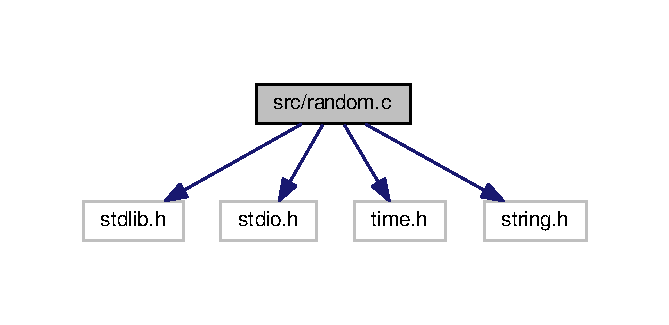
\includegraphics[width=322pt]{random_8c__incl}
\end{center}
\end{figure}
\subsection*{Fonctions}
\begin{DoxyCompactItemize}
\item 
\hypertarget{random_8c_affc667f54d3aad05a212a708a1967851}{void \hyperlink{random_8c_affc667f54d3aad05a212a708a1967851}{init\+Rand} ()}\label{random_8c_affc667f54d3aad05a212a708a1967851}

\begin{DoxyCompactList}\small\item\em Initialise le tirage aléatoire. \end{DoxyCompactList}\item 
char \hyperlink{random_8c_ab34a3eb028740a3f61ce69c5efaac376}{rand\+Char} ()
\begin{DoxyCompactList}\small\item\em Tire une lettre au hasard en prenant en compte leur fréquence d'apparition dans la langue française. \end{DoxyCompactList}\item 
int \hyperlink{random_8c_a8de3f80b9cac15b21aee0c7d56ae0f5a}{get\+I\+Char} (char c)
\begin{DoxyCompactList}\small\item\em Permet de récupérer l'indice dans la matrice de la lettre tirée au hasard. \end{DoxyCompactList}\item 
int \hyperlink{random_8c_a92316f4f4339b1dd0436637ce9552bb6}{rand\+Case} ()
\begin{DoxyCompactList}\small\item\em Permet de tirer une lettre aléatoirement. \end{DoxyCompactList}\item 
void \hyperlink{random_8c_a9b2c6b2bb8b813fc92d7f8be99e5d47d}{get\+Bonus} (char bo\+Char\+L\mbox{[}$\,$\mbox{]}, char bo\+Char\+M\mbox{[}$\,$\mbox{]}, int $\ast$nb\+\_\+bo\+L, int $\ast$nb\+\_\+bo\+M)
\begin{DoxyCompactList}\small\item\em Attribue un bonus. \end{DoxyCompactList}\end{DoxyCompactItemize}


\subsection{Description détaillée}
Fonctions aléatoires. 

\begin{DoxyAuthor}{Auteur}
Cousin Brandon Ngatchou Junior 
\end{DoxyAuthor}
\begin{DoxyVersion}{Version}
v1.\+00 
\end{DoxyVersion}
\begin{DoxyDate}{Date}
05/11/2015 
\end{DoxyDate}


Définition dans le fichier \hyperlink{random_8c_source}{random.\+c}.



\subsection{Documentation des fonctions}
\hypertarget{random_8c_a9b2c6b2bb8b813fc92d7f8be99e5d47d}{\index{random.\+c@{random.\+c}!get\+Bonus@{get\+Bonus}}
\index{get\+Bonus@{get\+Bonus}!random.\+c@{random.\+c}}
\subsubsection[{get\+Bonus}]{\setlength{\rightskip}{0pt plus 5cm}void get\+Bonus (
\begin{DoxyParamCaption}
\item[{char}]{bo\+Char\+L\mbox{[}$\,$\mbox{]}, }
\item[{char}]{bo\+Char\+M\mbox{[}$\,$\mbox{]}, }
\item[{int $\ast$}]{nb\+\_\+bo\+L, }
\item[{int $\ast$}]{nb\+\_\+bo\+M}
\end{DoxyParamCaption}
)}}\label{random_8c_a9b2c6b2bb8b813fc92d7f8be99e5d47d}


Attribue un bonus. 


\begin{DoxyParams}{Paramètres}
{\em bo\+Char\+L\mbox{[}$\,$\mbox{]}} & Bonus lettre de la case courante \\
\hline
{\em bo\+Char\+M\mbox{[}$\,$\mbox{]}} & Bonus mot de la case courante \\
\hline
{\em nb\+\_\+bo\+L} & Nombre de bonus lettre dans la grille \\
\hline
{\em nb\+\_\+bo\+M} & Nombre de bonus mot dans la grille \\
\hline
\end{DoxyParams}


Définition à la ligne 82 du fichier random.\+c.

\hypertarget{random_8c_a8de3f80b9cac15b21aee0c7d56ae0f5a}{\index{random.\+c@{random.\+c}!get\+I\+Char@{get\+I\+Char}}
\index{get\+I\+Char@{get\+I\+Char}!random.\+c@{random.\+c}}
\subsubsection[{get\+I\+Char}]{\setlength{\rightskip}{0pt plus 5cm}int get\+I\+Char (
\begin{DoxyParamCaption}
\item[{char}]{c}
\end{DoxyParamCaption}
)}}\label{random_8c_a8de3f80b9cac15b21aee0c7d56ae0f5a}


Permet de récupérer l'indice dans la matrice de la lettre tirée au hasard. 


\begin{DoxyParams}{Paramètres}
{\em c} & Caractère à convertir en indice \\
\hline
\end{DoxyParams}


Définition à la ligne 63 du fichier random.\+c.

\hypertarget{random_8c_a92316f4f4339b1dd0436637ce9552bb6}{\index{random.\+c@{random.\+c}!rand\+Case@{rand\+Case}}
\index{rand\+Case@{rand\+Case}!random.\+c@{random.\+c}}
\subsubsection[{rand\+Case}]{\setlength{\rightskip}{0pt plus 5cm}int rand\+Case (
\begin{DoxyParamCaption}
{}
\end{DoxyParamCaption}
)}}\label{random_8c_a92316f4f4339b1dd0436637ce9552bb6}


Permet de tirer une lettre aléatoirement. 

\begin{DoxyReturn}{Renvoie}
Renvoie l'indice de la lettre tirée 
\end{DoxyReturn}


Définition à la ligne 71 du fichier random.\+c.

\hypertarget{random_8c_ab34a3eb028740a3f61ce69c5efaac376}{\index{random.\+c@{random.\+c}!rand\+Char@{rand\+Char}}
\index{rand\+Char@{rand\+Char}!random.\+c@{random.\+c}}
\subsubsection[{rand\+Char}]{\setlength{\rightskip}{0pt plus 5cm}char rand\+Char (
\begin{DoxyParamCaption}
{}
\end{DoxyParamCaption}
)}}\label{random_8c_ab34a3eb028740a3f61ce69c5efaac376}


Tire une lettre au hasard en prenant en compte leur fréquence d'apparition dans la langue française. 

\begin{DoxyReturn}{Renvoie}
e par défaut 
\end{DoxyReturn}


Définition à la ligne 27 du fichier random.\+c.


\hypertarget{ruzzle_8c}{\section{Référence du fichier src/ruzzle.c}
\label{ruzzle_8c}\index{src/ruzzle.\+c@{src/ruzzle.\+c}}
}


Solver de Ruzzle.  


{\ttfamily \#include $<$stdio.\+h$>$}\\*
{\ttfamily \#include $<$stdlib.\+h$>$}\\*
{\ttfamily \#include \char`\"{}../include/display.\+h\char`\"{}}\\*
{\ttfamily \#include \char`\"{}../include/solver.\+h\char`\"{}}\\*
{\ttfamily \#include \char`\"{}../include/trie.\+h\char`\"{}}\\*
Graphe des dépendances par inclusion de ruzzle.\+c\+:\nopagebreak
\begin{figure}[H]
\begin{center}
\leavevmode
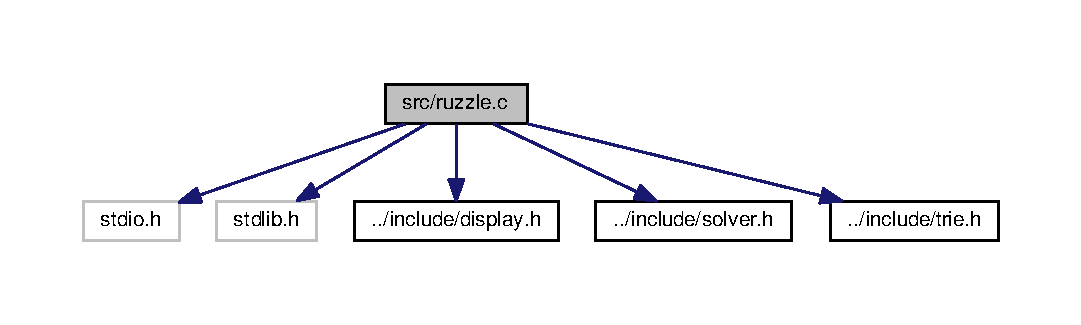
\includegraphics[width=350pt]{ruzzle_8c__incl}
\end{center}
\end{figure}
\subsection*{Fonctions}
\begin{DoxyCompactItemize}
\item 
\hypertarget{ruzzle_8c_a0ddf1224851353fc92bfbff6f499fa97}{int \hyperlink{ruzzle_8c_a0ddf1224851353fc92bfbff6f499fa97}{main} (int argc, char $\ast$argv\mbox{[}$\,$\mbox{]})}\label{ruzzle_8c_a0ddf1224851353fc92bfbff6f499fa97}

\begin{DoxyCompactList}\small\item\em Programme principal. \end{DoxyCompactList}\end{DoxyCompactItemize}


\subsection{Description détaillée}
Solver de Ruzzle. 

\begin{DoxyAuthor}{Auteur}
Cousin Brandon Ngatchou Junior 
\end{DoxyAuthor}
\begin{DoxyVersion}{Version}
v1.\+00 
\end{DoxyVersion}
\begin{DoxyDate}{Date}
05/11/2015 
\end{DoxyDate}


Définition dans le fichier \hyperlink{ruzzle_8c_source}{ruzzle.\+c}.


\hypertarget{solver_8c}{\section{Référence du fichier src/solver.c}
\label{solver_8c}\index{src/solver.\+c@{src/solver.\+c}}
}


Résoud la grille.  


{\ttfamily \#include $<$stdio.\+h$>$}\\*
{\ttfamily \#include $<$stdlib.\+h$>$}\\*
{\ttfamily \#include $<$string.\+h$>$}\\*
{\ttfamily \#include \char`\"{}../include/display.\+h\char`\"{}}\\*
{\ttfamily \#include \char`\"{}../include/solver.\+h\char`\"{}}\\*
{\ttfamily \#include \char`\"{}../include/trie.\+h\char`\"{}}\\*
Graphe des dépendances par inclusion de solver.\+c\+:\nopagebreak
\begin{figure}[H]
\begin{center}
\leavevmode
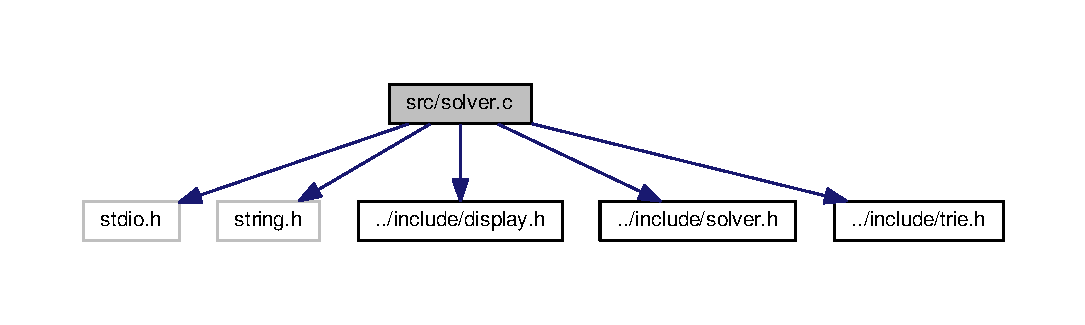
\includegraphics[width=350pt]{solver_8c__incl}
\end{center}
\end{figure}
\subsection*{Fonctions}
\begin{DoxyCompactItemize}
\item 
int \hyperlink{solver_8c_a07d68aeb0b5ed32ab93e34e1a8a2be44}{tot\+Case} (\hyperlink{structt__Case}{t\+\_\+\+Case} Case)
\begin{DoxyCompactList}\small\item\em Calcule le total de points de la case courante. \end{DoxyCompactList}\item 
int \hyperlink{solver_8c_a0b23cdd3365d624985e5123a2c0f9034}{mul\+Word} (\hyperlink{structt__Case}{t\+\_\+\+Case} Case)
\begin{DoxyCompactList}\small\item\em Retourne le coefficient multiplicateur pour le mot entier. \end{DoxyCompactList}\item 
char $\ast$ \hyperlink{solver_8c_ad6f794353350ca765c5176a821b8d0e5}{get\+Word} (F\+I\+L\+E $\ast$dict)
\begin{DoxyCompactList}\small\item\em Récupère un mot dans le dictionnaire. \end{DoxyCompactList}\item 
int \hyperlink{solver_8c_a9c6b017312dc83e7c70a60e8c984438a}{search\+Start} (\hyperlink{structt__Case}{t\+\_\+\+Case} Case, char word\mbox{[}$\,$\mbox{]})
\begin{DoxyCompactList}\small\item\em Cherche un point de départ à partir de la case courante. \end{DoxyCompactList}\item 
void \hyperlink{solver_8c_a22b87f42380ae5859ffcb636dc0689aa}{confirm\+Word} (char \hyperlink{solver_8c_ad03517614669b994d2153c8b5afe637b}{grid\+Word}\mbox{[}$\,$\mbox{]}, char word\mbox{[}$\,$\mbox{]}, int pts)
\begin{DoxyCompactList}\small\item\em Permet de confirmer que les deux mots sont identiques si c'est le cas alors on le rajoute dans la liste chaînée. \end{DoxyCompactList}\item 
void \hyperlink{solver_8c_acbb5df3f19b52b649ee3d8ac41c90795}{form\+Word} (\hyperlink{structt__Case}{t\+\_\+\+Case} grid\mbox{[}\hyperlink{display_8h_a0240ac851181b84ac374872dc5434ee4}{N}\mbox{]}\mbox{[}\hyperlink{display_8h_a0240ac851181b84ac374872dc5434ee4}{N}\mbox{]}, int i, int j, char word\mbox{[}$\,$\mbox{]})
\begin{DoxyCompactList}\small\item\em Forme un mot en parcourant la grille. \end{DoxyCompactList}\item 
void \hyperlink{solver_8c_a304c6271abc4ca96f7341762845cfb90}{search\+Word} (\hyperlink{structt__Case}{t\+\_\+\+Case} grid\mbox{[}\hyperlink{display_8h_a0240ac851181b84ac374872dc5434ee4}{N}\mbox{]}\mbox{[}\hyperlink{display_8h_a0240ac851181b84ac374872dc5434ee4}{N}\mbox{]}, char word\mbox{[}$\,$\mbox{]})
\begin{DoxyCompactList}\small\item\em Cherche le mot dans la grille. \end{DoxyCompactList}\item 
void \hyperlink{solver_8c_acb26ab357db8918adfe55385af56ba11}{Solver} (\hyperlink{structt__Case}{t\+\_\+\+Case} grid\mbox{[}\hyperlink{display_8h_a0240ac851181b84ac374872dc5434ee4}{N}\mbox{]}\mbox{[}\hyperlink{display_8h_a0240ac851181b84ac374872dc5434ee4}{N}\mbox{]})
\begin{DoxyCompactList}\small\item\em Résoud la grille. \end{DoxyCompactList}\end{DoxyCompactItemize}
\subsection*{Variables}
\begin{DoxyCompactItemize}
\item 
\hypertarget{solver_8c_ad03517614669b994d2153c8b5afe637b}{char \hyperlink{solver_8c_ad03517614669b994d2153c8b5afe637b}{grid\+Word} \mbox{[}17\mbox{]} = \char`\"{}\textbackslash{}0\char`\"{}}\label{solver_8c_ad03517614669b994d2153c8b5afe637b}

\begin{DoxyCompactList}\small\item\em Mot formé à partir de la grille. \end{DoxyCompactList}\item 
\hypertarget{solver_8c_ab44c51dc8f611c449d8b69d2e9f8f1d5}{int \hyperlink{solver_8c_ab44c51dc8f611c449d8b69d2e9f8f1d5}{total\+W} = 0}\label{solver_8c_ab44c51dc8f611c449d8b69d2e9f8f1d5}

\begin{DoxyCompactList}\small\item\em Total points du mot formé \end{DoxyCompactList}\item 
\hypertarget{solver_8c_ab43147501c62fb816bb6b5edea66cae1}{int \hyperlink{solver_8c_ab43147501c62fb816bb6b5edea66cae1}{bo\+W} = 1}\label{solver_8c_ab43147501c62fb816bb6b5edea66cae1}

\begin{DoxyCompactList}\small\item\em Bonus multiplicateur du mot. \end{DoxyCompactList}\end{DoxyCompactItemize}


\subsection{Description détaillée}
Résoud la grille. 

\begin{DoxyAuthor}{Auteur}
Cousin Brandon Ngatchou Junior 
\end{DoxyAuthor}
\begin{DoxyVersion}{Version}
v1.\+00 
\end{DoxyVersion}
\begin{DoxyDate}{Date}
08/11/2015 
\end{DoxyDate}


Définition dans le fichier \hyperlink{solver_8c_source}{solver.\+c}.



\subsection{Documentation des fonctions}
\hypertarget{solver_8c_a22b87f42380ae5859ffcb636dc0689aa}{\index{solver.\+c@{solver.\+c}!confirm\+Word@{confirm\+Word}}
\index{confirm\+Word@{confirm\+Word}!solver.\+c@{solver.\+c}}
\subsubsection[{confirm\+Word}]{\setlength{\rightskip}{0pt plus 5cm}void confirm\+Word (
\begin{DoxyParamCaption}
\item[{char}]{grid\+Word\mbox{[}$\,$\mbox{]}, }
\item[{char}]{word\mbox{[}$\,$\mbox{]}, }
\item[{int}]{pts}
\end{DoxyParamCaption}
)}}\label{solver_8c_a22b87f42380ae5859ffcb636dc0689aa}


Permet de confirmer que les deux mots sont identiques si c'est le cas alors on le rajoute dans la liste chaînée. 


\begin{DoxyParams}{Paramètres}
{\em grid\+Word} & Mot formé à partir de la grille \\
\hline
{\em word} & Mot tiré du dictionnaire \\
\hline
{\em pts} & Nombre de points total pour le mot formé \\
\hline
\end{DoxyParams}


Définition à la ligne 73 du fichier solver.\+c.

\hypertarget{solver_8c_acbb5df3f19b52b649ee3d8ac41c90795}{\index{solver.\+c@{solver.\+c}!form\+Word@{form\+Word}}
\index{form\+Word@{form\+Word}!solver.\+c@{solver.\+c}}
\subsubsection[{form\+Word}]{\setlength{\rightskip}{0pt plus 5cm}void form\+Word (
\begin{DoxyParamCaption}
\item[{{\bf t\+\_\+\+Case}}]{grid\mbox{[}\+N\mbox{]}\mbox{[}\+N\mbox{]}, }
\item[{int}]{i, }
\item[{int}]{j, }
\item[{char}]{word\mbox{[}$\,$\mbox{]}}
\end{DoxyParamCaption}
)}}\label{solver_8c_acbb5df3f19b52b649ee3d8ac41c90795}


Forme un mot en parcourant la grille. 


\begin{DoxyParams}{Paramètres}
{\em grid} & Grille à résoudre \\
\hline
{\em i} & Point de départ vertical \\
\hline
{\em j} & Point de départ horizontal \\
\hline
{\em word} & Mot à chercher \\
\hline
\end{DoxyParams}


Définition à la ligne 91 du fichier solver.\+c.

\hypertarget{solver_8c_ad6f794353350ca765c5176a821b8d0e5}{\index{solver.\+c@{solver.\+c}!get\+Word@{get\+Word}}
\index{get\+Word@{get\+Word}!solver.\+c@{solver.\+c}}
\subsubsection[{get\+Word}]{\setlength{\rightskip}{0pt plus 5cm}char$\ast$ get\+Word (
\begin{DoxyParamCaption}
\item[{F\+I\+L\+E $\ast$}]{dict}
\end{DoxyParamCaption}
)}}\label{solver_8c_ad6f794353350ca765c5176a821b8d0e5}


Récupère un mot dans le dictionnaire. 


\begin{DoxyParams}{Paramètres}
{\em dict} & Dictionnaire dans lequel regarder \\
\hline
\end{DoxyParams}
\begin{DoxyReturn}{Renvoie}
Retourne un mot dans l'ordre séquentiel 
\end{DoxyReturn}


Définition à la ligne 47 du fichier solver.\+c.

\hypertarget{solver_8c_a0b23cdd3365d624985e5123a2c0f9034}{\index{solver.\+c@{solver.\+c}!mul\+Word@{mul\+Word}}
\index{mul\+Word@{mul\+Word}!solver.\+c@{solver.\+c}}
\subsubsection[{mul\+Word}]{\setlength{\rightskip}{0pt plus 5cm}int mul\+Word (
\begin{DoxyParamCaption}
\item[{{\bf t\+\_\+\+Case}}]{Case}
\end{DoxyParamCaption}
)}}\label{solver_8c_a0b23cdd3365d624985e5123a2c0f9034}


Retourne le coefficient multiplicateur pour le mot entier. 


\begin{DoxyParams}{Paramètres}
{\em Case} & Case courante \\
\hline
\end{DoxyParams}
\begin{DoxyReturn}{Renvoie}
1 si pas de bonus, 2 si bonus double, 3 si bonus triple 
\end{DoxyReturn}


Définition à la ligne 36 du fichier solver.\+c.

\hypertarget{solver_8c_a9c6b017312dc83e7c70a60e8c984438a}{\index{solver.\+c@{solver.\+c}!search\+Start@{search\+Start}}
\index{search\+Start@{search\+Start}!solver.\+c@{solver.\+c}}
\subsubsection[{search\+Start}]{\setlength{\rightskip}{0pt plus 5cm}int search\+Start (
\begin{DoxyParamCaption}
\item[{{\bf t\+\_\+\+Case}}]{Case, }
\item[{char}]{word\mbox{[}$\,$\mbox{]}}
\end{DoxyParamCaption}
)}}\label{solver_8c_a9c6b017312dc83e7c70a60e8c984438a}


Cherche un point de départ à partir de la case courante. 


\begin{DoxyParams}{Paramètres}
{\em Case} & Case courante \\
\hline
{\em word} & Mot récupéré dans le dictionnaire \\
\hline
\end{DoxyParams}
\begin{DoxyReturn}{Renvoie}
Retourne 1 si point de départ trouvé sinon 0 
\end{DoxyReturn}


Définition à la ligne 62 du fichier solver.\+c.

\hypertarget{solver_8c_a304c6271abc4ca96f7341762845cfb90}{\index{solver.\+c@{solver.\+c}!search\+Word@{search\+Word}}
\index{search\+Word@{search\+Word}!solver.\+c@{solver.\+c}}
\subsubsection[{search\+Word}]{\setlength{\rightskip}{0pt plus 5cm}void search\+Word (
\begin{DoxyParamCaption}
\item[{{\bf t\+\_\+\+Case}}]{grid\mbox{[}\+N\mbox{]}\mbox{[}\+N\mbox{]}, }
\item[{char}]{word\mbox{[}$\,$\mbox{]}}
\end{DoxyParamCaption}
)}}\label{solver_8c_a304c6271abc4ca96f7341762845cfb90}


Cherche le mot dans la grille. 


\begin{DoxyParams}{Paramètres}
{\em grid} & Grille à résoudre \\
\hline
{\em word} & Mot récupéré dans le dictionnaire \\
\hline
\end{DoxyParams}


Définition à la ligne 130 du fichier solver.\+c.

\hypertarget{solver_8c_acb26ab357db8918adfe55385af56ba11}{\index{solver.\+c@{solver.\+c}!Solver@{Solver}}
\index{Solver@{Solver}!solver.\+c@{solver.\+c}}
\subsubsection[{Solver}]{\setlength{\rightskip}{0pt plus 5cm}void Solver (
\begin{DoxyParamCaption}
\item[{{\bf t\+\_\+\+Case}}]{grid\mbox{[}\+N\mbox{]}\mbox{[}\+N\mbox{]}}
\end{DoxyParamCaption}
)}}\label{solver_8c_acb26ab357db8918adfe55385af56ba11}


Résoud la grille. 


\begin{DoxyParams}{Paramètres}
{\em grid} & Grille à résoudre \\
\hline
\end{DoxyParams}


Définition à la ligne 148 du fichier solver.\+c.

\hypertarget{solver_8c_a07d68aeb0b5ed32ab93e34e1a8a2be44}{\index{solver.\+c@{solver.\+c}!tot\+Case@{tot\+Case}}
\index{tot\+Case@{tot\+Case}!solver.\+c@{solver.\+c}}
\subsubsection[{tot\+Case}]{\setlength{\rightskip}{0pt plus 5cm}int tot\+Case (
\begin{DoxyParamCaption}
\item[{{\bf t\+\_\+\+Case}}]{Case}
\end{DoxyParamCaption}
)}}\label{solver_8c_a07d68aeb0b5ed32ab93e34e1a8a2be44}


Calcule le total de points de la case courante. 


\begin{DoxyParams}{Paramètres}
{\em Case} & Case courante \\
\hline
\end{DoxyParams}
\begin{DoxyReturn}{Renvoie}
Le nombre de points total 
\end{DoxyReturn}


Définition à la ligne 25 du fichier solver.\+c.


\hypertarget{trie_8c}{\section{Référence du fichier src/trie.c}
\label{trie_8c}\index{src/trie.\+c@{src/trie.\+c}}
}


Met au point une liste chaînée d'ordre décroissant.  


{\ttfamily \#include $<$stdio.\+h$>$}\\*
{\ttfamily \#include $<$stdlib.\+h$>$}\\*
{\ttfamily \#include $<$string.\+h$>$}\\*
{\ttfamily \#include \char`\"{}../include/trie.\+h\char`\"{}}\\*
Graphe des dépendances par inclusion de trie.\+c\+:\nopagebreak
\begin{figure}[H]
\begin{center}
\leavevmode
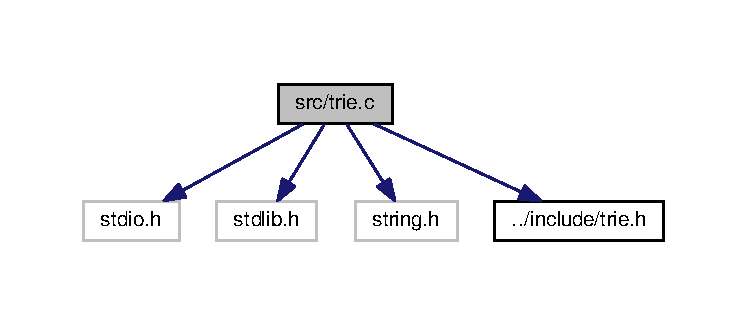
\includegraphics[width=350pt]{trie_8c__incl}
\end{center}
\end{figure}
\subsection*{Fonctions}
\begin{DoxyCompactItemize}
\item 
void \hyperlink{trie_8c_adac30872b2982daea2a38df6f042065d}{add\+Element} (\hyperlink{structelement}{element} $\ast$elem)
\begin{DoxyCompactList}\small\item\em Ajoute un élément dans la liste chaînée. \end{DoxyCompactList}\item 
\hypertarget{trie_8c_a2f736094bbaa598f70c3e241bad4a1cc}{void \hyperlink{trie_8c_a2f736094bbaa598f70c3e241bad4a1cc}{print\+List} ()}\label{trie_8c_a2f736094bbaa598f70c3e241bad4a1cc}

\begin{DoxyCompactList}\small\item\em Affiche la liste entière de la racine jusqu'à la fin. \end{DoxyCompactList}\item 
\hypertarget{trie_8c_a612285c5b9d603a0abb0feab44b8412f}{void \hyperlink{trie_8c_a612285c5b9d603a0abb0feab44b8412f}{clear\+List} ()}\label{trie_8c_a612285c5b9d603a0abb0feab44b8412f}

\begin{DoxyCompactList}\small\item\em Supprime la liste. \end{DoxyCompactList}\end{DoxyCompactItemize}
\subsection*{Variables}
\begin{DoxyCompactItemize}
\item 
\hypertarget{trie_8c_a400fc15964edd9c35132913b24b25ded}{\hyperlink{structelement}{element} $\ast$ \hyperlink{trie_8c_a400fc15964edd9c35132913b24b25ded}{root} = N\+U\+L\+L}\label{trie_8c_a400fc15964edd9c35132913b24b25ded}

\begin{DoxyCompactList}\small\item\em Définis la racine de la liste chaînée. \end{DoxyCompactList}\end{DoxyCompactItemize}


\subsection{Description détaillée}
Met au point une liste chaînée d'ordre décroissant. 

\begin{DoxyAuthor}{Auteur}
Cousin Brandon Ngatchou Junior 
\end{DoxyAuthor}
\begin{DoxyVersion}{Version}
v1.\+00 
\end{DoxyVersion}
\begin{DoxyDate}{Date}
08/11/2015 
\end{DoxyDate}


Définition dans le fichier \hyperlink{trie_8c_source}{trie.\+c}.



\subsection{Documentation des fonctions}
\hypertarget{trie_8c_adac30872b2982daea2a38df6f042065d}{\index{trie.\+c@{trie.\+c}!add\+Element@{add\+Element}}
\index{add\+Element@{add\+Element}!trie.\+c@{trie.\+c}}
\subsubsection[{add\+Element}]{\setlength{\rightskip}{0pt plus 5cm}void add\+Element (
\begin{DoxyParamCaption}
\item[{{\bf element} $\ast$}]{elem}
\end{DoxyParamCaption}
)}}\label{trie_8c_adac30872b2982daea2a38df6f042065d}


Ajoute un élément dans la liste chaînée. 


\begin{DoxyParams}{Paramètres}
{\em elem} & Elément à ajouter \\
\hline
\end{DoxyParams}


Définition à la ligne 20 du fichier trie.\+c.


%--- End generated contents ---

% Index
\newpage
\phantomsection
\addcontentsline{toc}{chapter}{Index}
\printindex

\end{document}
